\documentclass{beamer}

% \usepackage{beamerthemesplit} // Activate for custom appearance

\title{Building Artificial Life and Multi-Agent simulations using the Breve engine}
\author{Wouter Bulten, Frank Dorssers \& Robert-Jan Drenth}
\date{\textit{ACAIS: Life}, June 6th 2013}

\usebackgroundtemplate{%
  \vbox to 1.8\paperheight{\vfil\hbox to 1.66\paperwidth{\hfil
\includegraphics[height=0.4in]{ACAIS2013_logodatum}\hfil}\vfil}

}
\definecolor{acaisred}{rgb}{0.75,0.19,0.1}

\setbeamercolor{title}{fg=acaisred}
\setbeamercolor{frametitle}{fg=acaisred}
\setbeamercolor{structure}{fg=acaisred}

\begin{document}

\frame{
\titlepage}

\frame{
	\frametitle{Goal of today}
	
	Investigating and building multi-agent and artificial life simulations.
	\begin{center}
		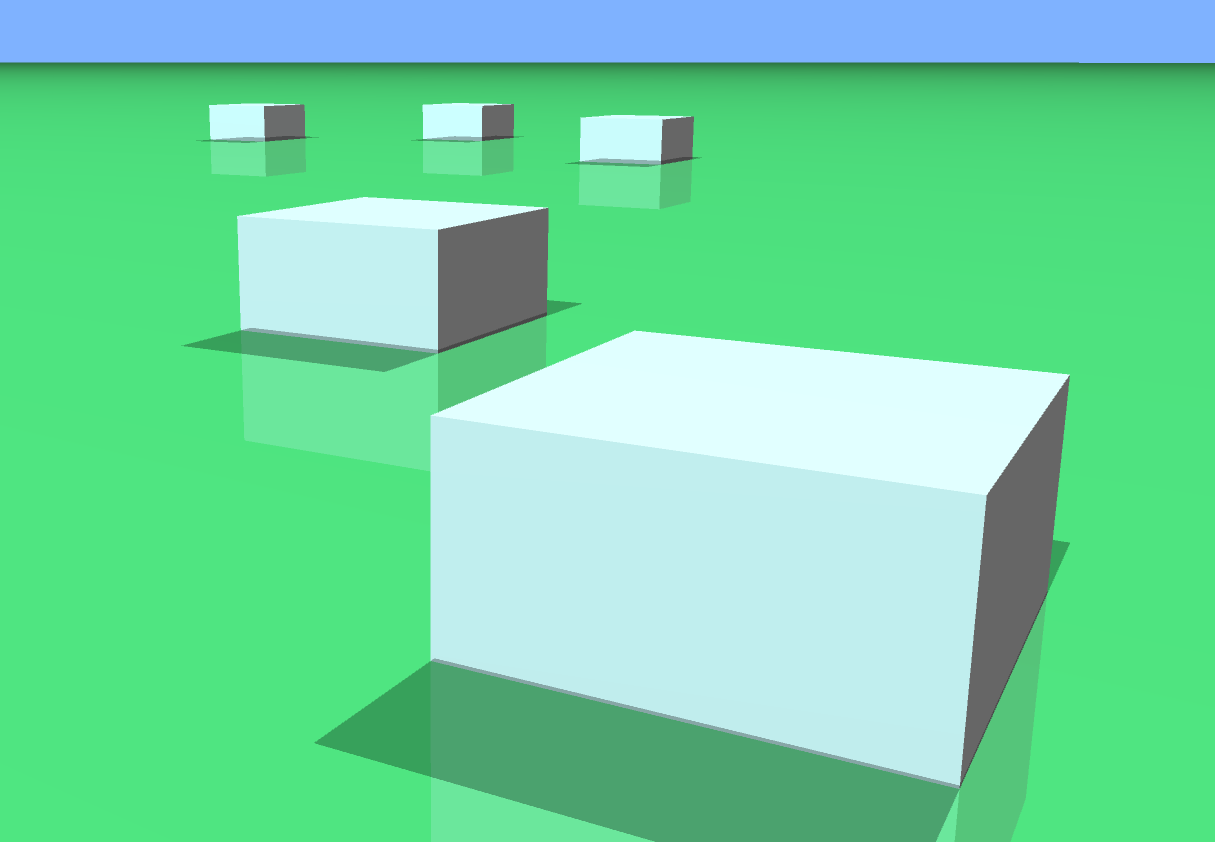
\includegraphics[width=0.5\textwidth]{agents.png}
	\end{center}
}

\section[Outline]{}
\frame{
\frametitle{Overview}
\tableofcontents}


\section{Introducing breve}
\frame{
	\frametitle{What is breve?}

\begin{columns}
	
	\column{0.7\textwidth}
	\begin{itemize}
		\item Environment designed for simulation of realistic, 3D, multi-agent systems
		\item Created by Jon Klein (Hampshire College \& Chalmers University)
		\item Autonomous agents
	\end{itemize}
	
	\column{0.3\textwidth}
	
	
\includegraphics[width=\textwidth]{breve_icon}

\end{columns}
}
\frame{
	\frametitle{Types of simulation}
	
	\begin{itemize}
		\item Multi-agent Simulations
		\item 3D spatial simulation
		\item Physical simulation 
	\end{itemize}
}
\frame{
	\frametitle{Why breve?}
	
	\begin{itemize}
		\item Easy way to visualise a simulation (and to disable it)
		\item Framework
		\item Open Source / Free to use
	\end{itemize}
}
\section{Past projects}

\frame{
	\frametitle{The evolution of leadership}
	
	\center {
		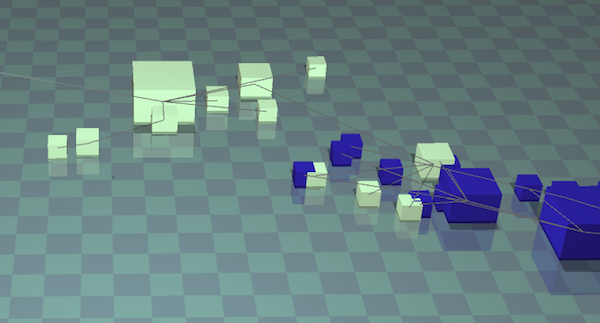
\includegraphics[width=\textwidth]{evolea}
	}
	{\tiny Wouter Bulten, Robert-Jan Drenth \& Lysanne Sloff}
}
\frame{
	\frametitle{Punishment Mechanisms and their Effect on Cooperation}
	\center {
		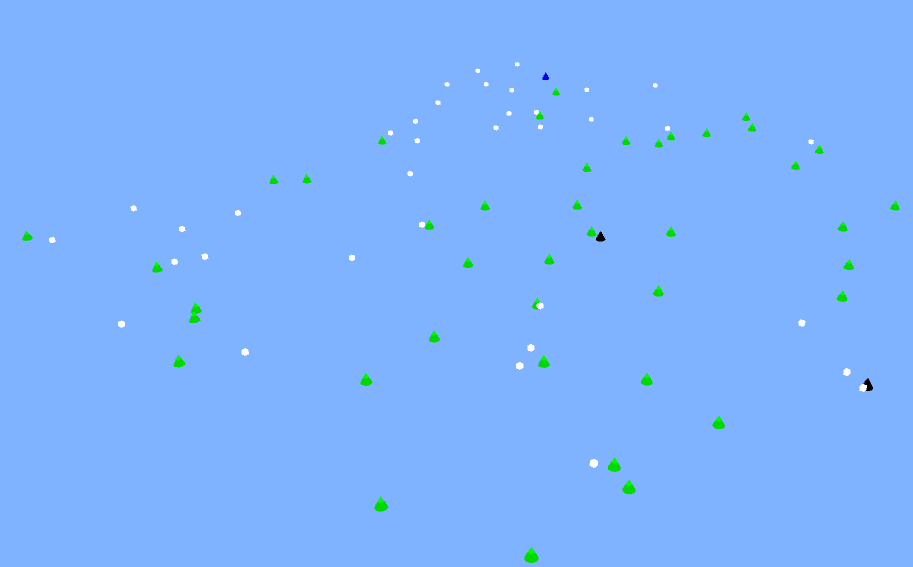
\includegraphics[width=\textwidth]{brevemike}
	}
	{\tiny Mike Farjam, Pim Haselager \& Ida Sprinkhuizen-Kuyper, BNAIC 2012}
}
\frame{
	\frametitle{Braitenberg}
	\center {
		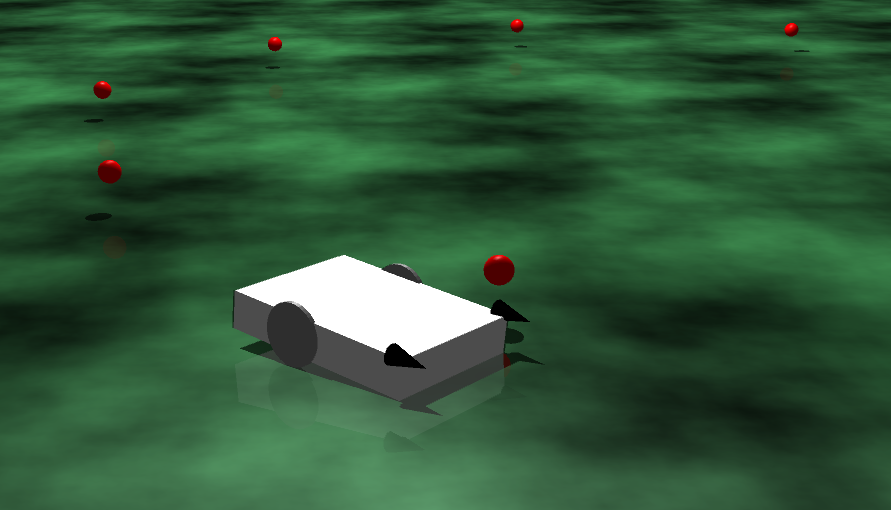
\includegraphics[width=\textwidth]{Braitenberg}
	}
}
\frame{
	\frametitle{Virtual Creatures}
	\center {
		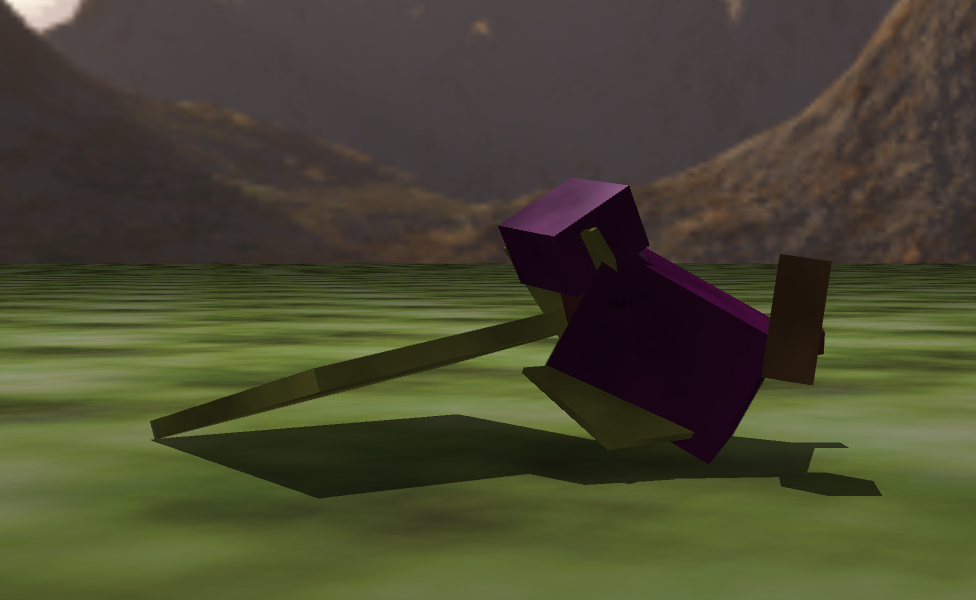
\includegraphics[width=\textwidth]{evolvewalker}
	}
	{\tiny Evolving virtual creatures, Sims (1994)}
}
\frame{
	\frametitle{Molecule}
	\center {
		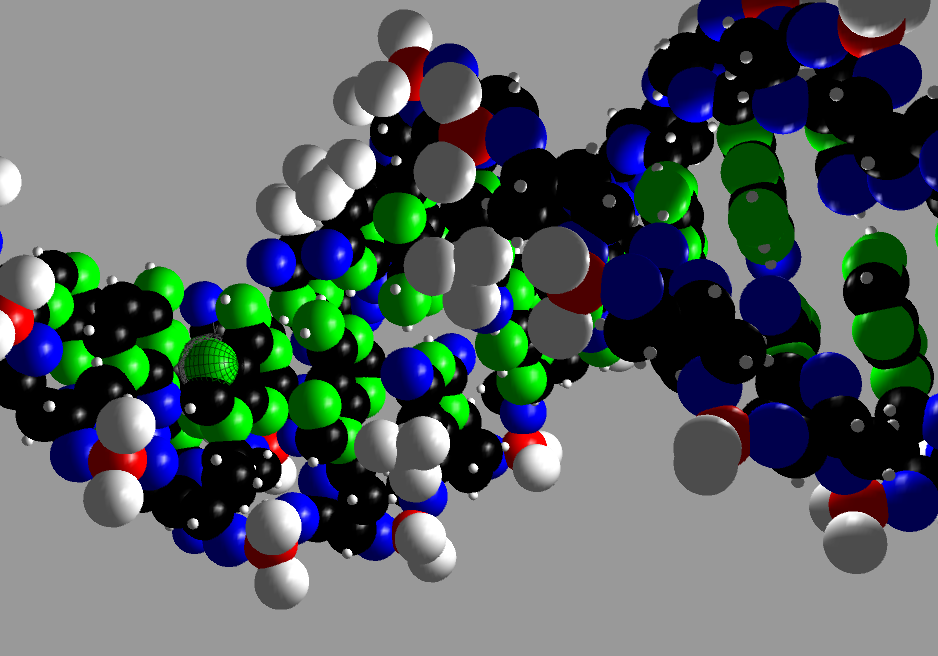
\includegraphics[width=\textwidth]{molecule}
	}
}
\frame{
	\frametitle{Sharing eco-system}
	
	\center {
		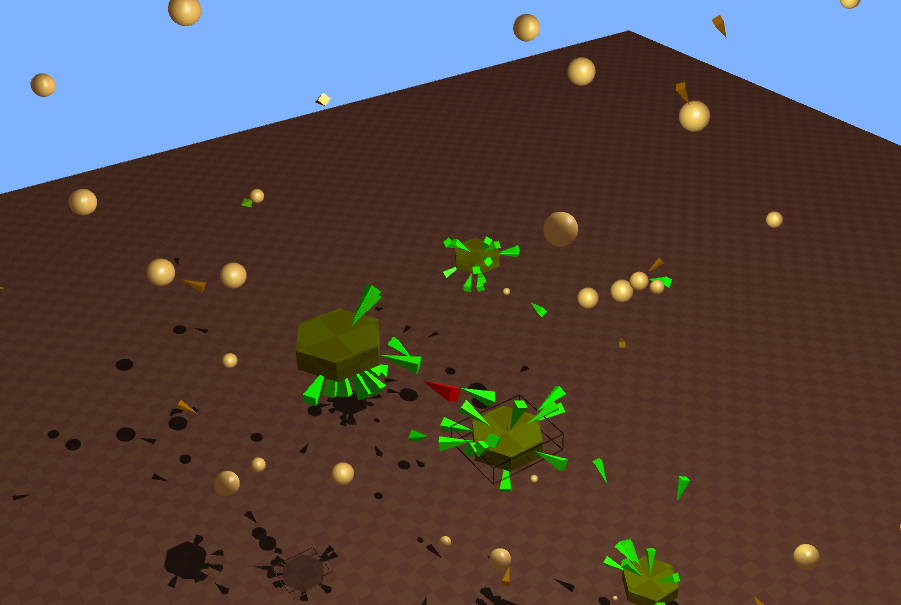
\includegraphics[width=\textwidth]{sharingeco}
	}
	
	{\tiny Wouter Bulten, Pim Haselager \& Ida Sprinkhuizen-Kuyper, BNAIC 2012}
}

\section{Basis of a simulation}
\frame{

	\frametitle{Basis of a simulation}
	
	Every simulation has the same building blocks:
	\begin{enumerate}
		\item Controller
		\item Agents
		\item Objects (floor, food, nests, etc.)
	\end{enumerate}
}

\section{Building a simulation}
\frame{

	
}

\section{Adding complexity}
\frame{
	\frametitle{Adding complexity}
	\begin{itemize}
		\item Communication between
			\begin{itemize}
				\item  agents (groups, leaders, followers)
				\item  simulations via a network
			\end{itemize}
		\item Use physics
		\item Add evolution/genetics (own modules, link with JGap, or built-in engine Push)
	\end{itemize}
}

\section{What we are going to build}
\frame{
	\frametitle{What we are going to build}
	
	\begin{columns}
	\column{0.5\textwidth}
	\begin{itemize}
		\item 3D decentralised food gathering algorithm
		\item No communication between agents
		\item Goal: collect food and make piles
		\item Optional: two groups
	\end{itemize}	
	
	\column{0.6\textwidth}
	
	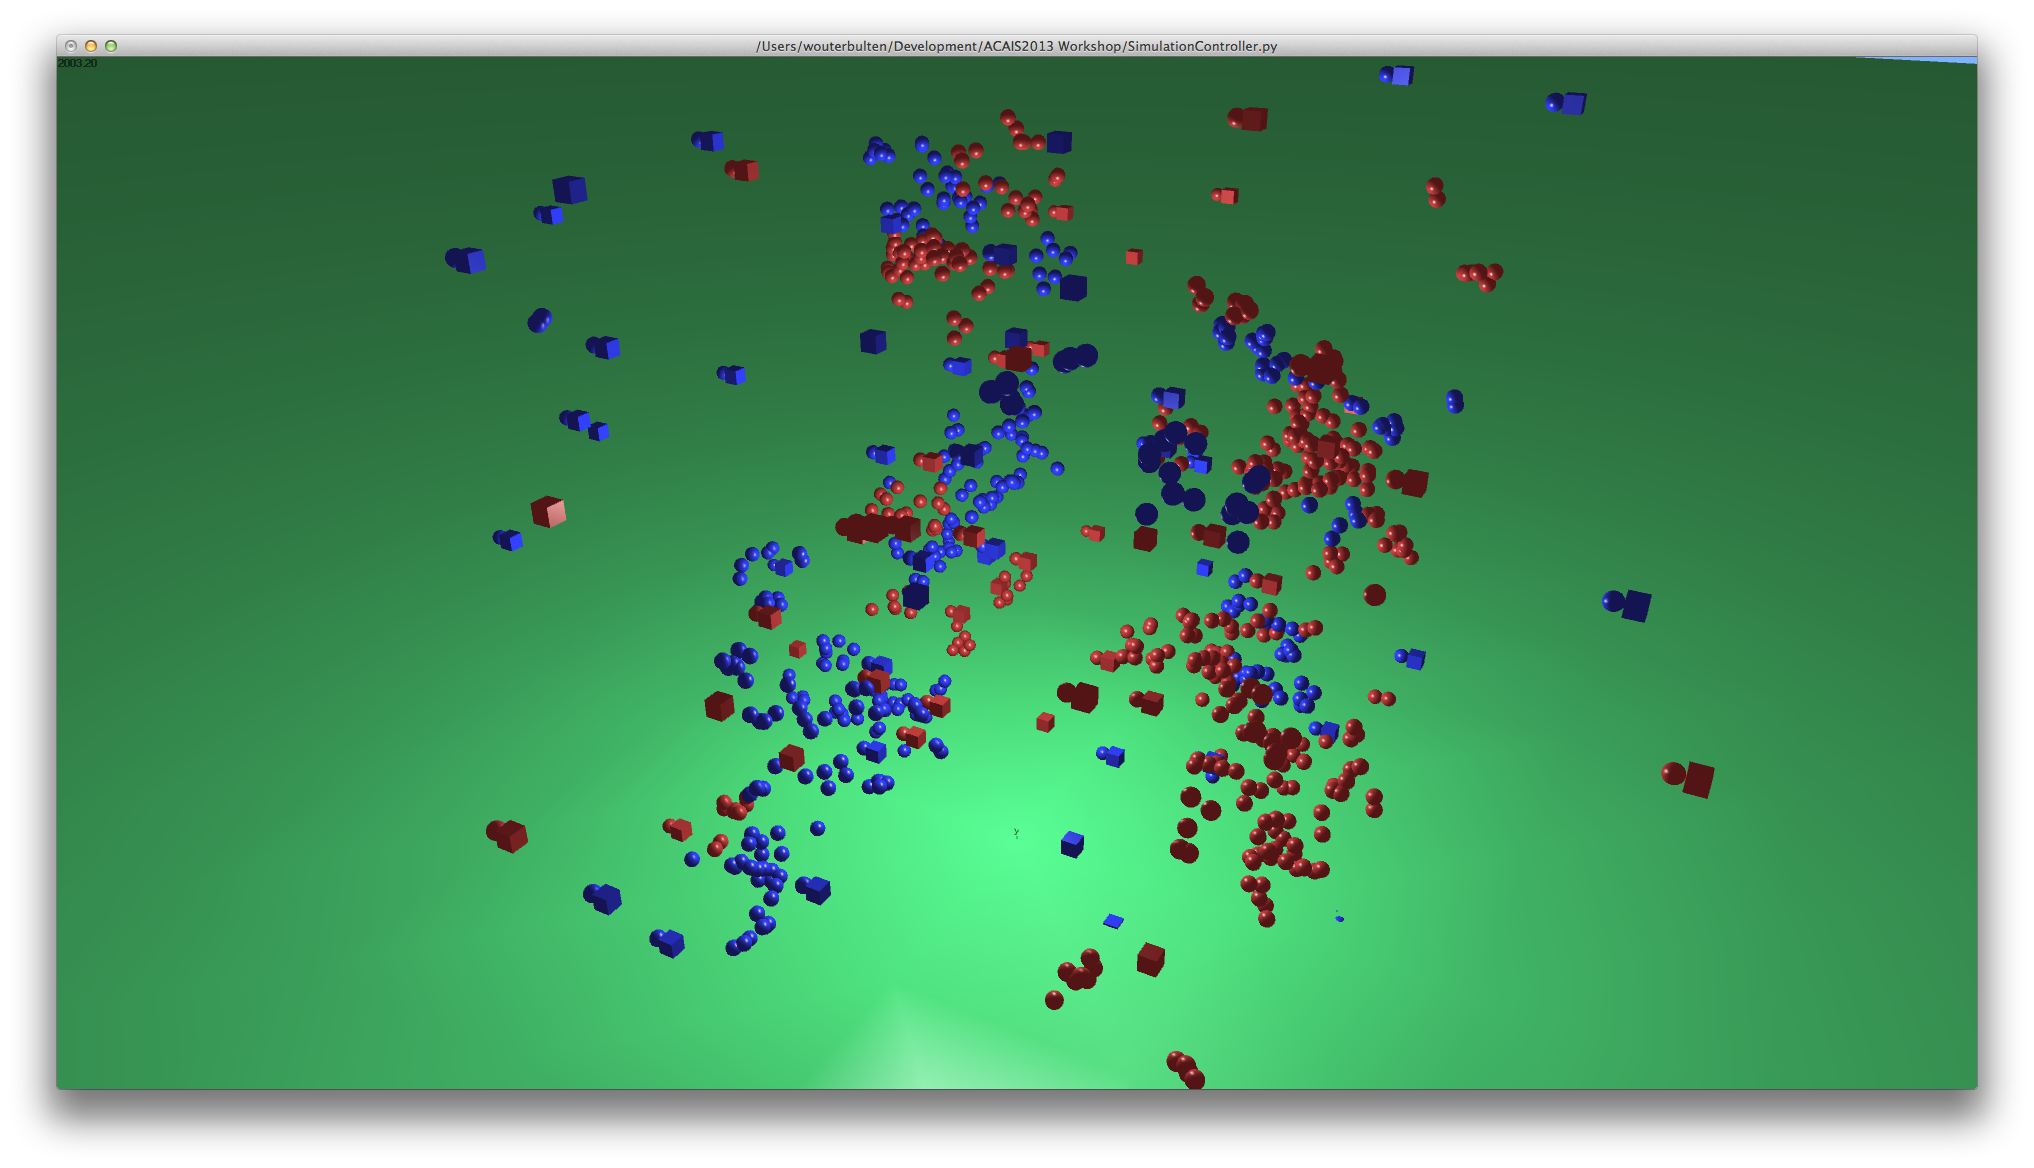
\includegraphics[width=\textwidth]{endproduct}

\end{columns}
}
\end{document}
